
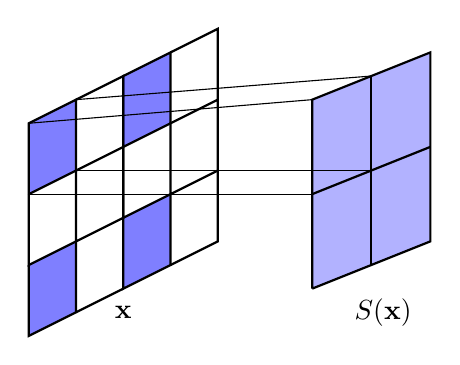
\begin{tikzpicture}[scale=0.6]
%\draw[opacity=0.5] (-4,-4) grid (4,4);

%%% grosse image

    % BLOCK (1,1)
% pixels bleu
\draw[thick, fill=blue, fill opacity=0.5] (-3,0) -- (-3,-1.5) -- (-4,-2)  -- (-4,-0.5);

% pixels blancs
\draw[thick, xshift=1cm, yshift=0.5cm] (-4,-2) -- (-3,-1.5);


    % BLOCK (2,1)
% pixels bleu
\draw[thick, fill=blue, fill opacity=0.5, xshift=2cm, yshift=1cm] (-3,0) -- (-3,-1.5) -- (-4,-2)  -- (-4,-0.5);

% pixels blancs
\draw[thick, xshift=3cm, yshift=1.5cm] (-3,0) -- (-3,-1.5) -- (-4,-2);

    % BLOCK (1,2)
% pixels bleu
\draw[thick, fill=blue, fill opacity=0.5, yshift=3cm] (-4,-2) -- (-4,-0.5) -- (-3,0) -- (-3,-1.5) -- (-4,-2);

% pixels blancs
\draw[thick, yshift=1.5cm] (-4,-0.5) -- (-4,-2) -- (-3,-1.5);
\draw[thick, xshift=1cm, yshift=3.5cm] (-4,-0.5) -- (-3,0) -- (-3,-1.5);

%pixels rouge
\draw[thick, xshift=1cm, yshift=2cm] (-4,-2) -- (-4,-0.5) -- (-3,0) -- (-3,-1.5) -- (-4,-2);

    % BLOCK (2,2)
% pixels bleu
\draw[thick, fill=blue, fill opacity=0.5, xshift=2cm, yshift=4cm] (-4,-2) -- (-4,-0.5) -- (-3,0) -- (-3,-1.5) -- (-4,-2);

% pixels blancs
\draw[thick, xshift=2cm, yshift=2.5cm] (-4,-0.5) -- (-4,-2) -- (-3,-1.5);
\draw[thick, xshift=3cm, yshift=4.5cm] (-4,-0.5) -- (-3,0) -- (-3,-1.5);

%pixels rouge
\draw[thick, xshift=3cm, yshift=3cm] (-4,-2) -- (-4,-0.5) -- (-3,0) -- (-3,-1.5) -- (-4,-2);

%%% petite image

\draw[thick, fill=blue, fill opacity=0.3, xshift=1cm] (1,-1) -- (1,3) -- (3.5,4) -- (3.5,0) -- (1,-1);
\draw[thick, xshift=2.25cm, yshift=0.5cm] (1,-1) -- (1,3);
\draw[thick, xshift=1cm, yshift=-2cm] (1,3) -- (3.5,4);

%%% lien

\draw (-4,1) -- (2,1);
\draw (-4,2.5) -- (2,3);
\draw (-3,1.5) -- (3.25,1.5);
\draw (-3,3) -- (3.25,3.5);

%%% Nom

\draw  (-2,-1.5) -- (-2,-1.5) node{$\bf{x}$};
\draw  (3.5,-1.5) -- (3.5,-1.5) node{$S(\bf{x})$};
\end{tikzpicture}